
\begin{appendix}


\chapter{Architecture des messages} \label{annexe}

Légende :
\begin{itemize}
    \item  Chaque carré bleu correspond à ce qui est contenu dans
    le fichier proto dont le nom est marqué dedans.
    \item Il y a forcément au minimum un \textbf{GC\_Msg} ou
    \textbf{Robot\_Message}, c'est pourquoi il sont en orange.
     \item Les éléments en rouge sont "required", en effet, si on
     prend le début du message, il est normal que chaque message
     ait un identifiant.
    \item Les fichiers en vert sont "repeated", en effet, on a
    plusieurs Message. Dans chaque message on va avoir plusieurs
    équipes et robots (donc \textbf{GCTeamMsg} et
    \textbf{GCRobotMsg} sont en vert).
    \item Enfin, les éléments en jaune sont optionnels.
    \item La position définie dans le fichier
    \textit{position.proto} est réutilisée dans tous les éléments
    où l'on voit le "\textasciitilde". 

\end{itemize}
\bigskip

L'architecture de ces messages a été définit par le client. Ce
schéma représentant l'architecture a été fait dès le début et nous
a beaucoup aidé à savoir comment sont hiérarchisés les messages.
    
\begin{figure}
    \centering
    \rotatebox{90}{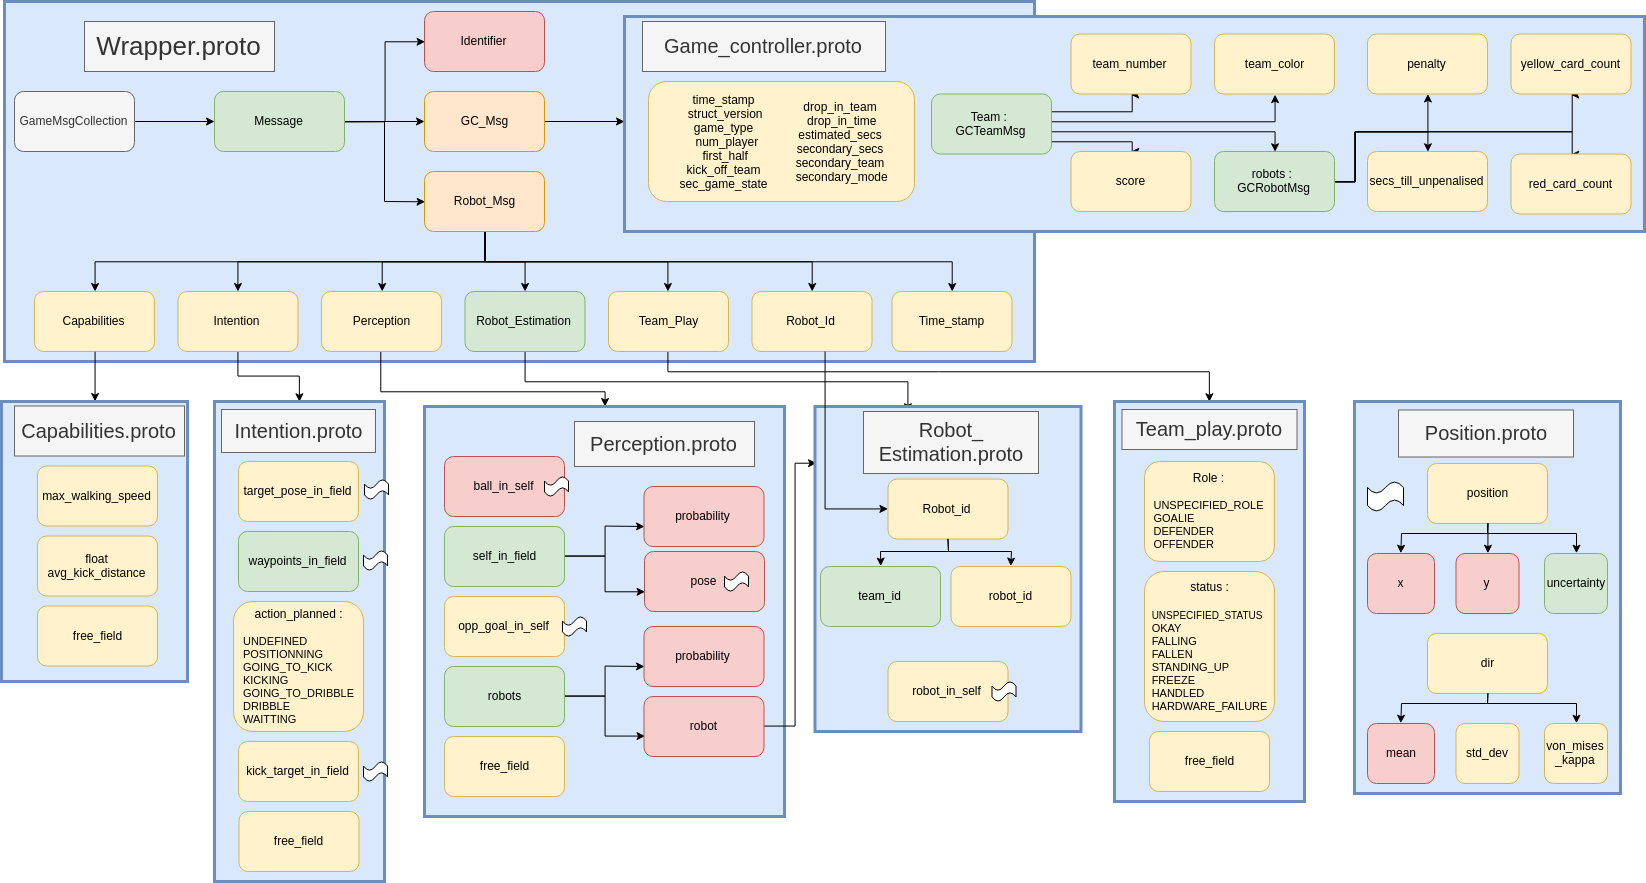
\includegraphics[scale = 0.35]{images/messages.png}}
    \label{fig:my_label}
\end{figure}

\end{appendix}
